%% The following is a directive for TeXShop to indicate the main file
%%!TEX root =../diss.tex

\chapter{Future Work}
\label{ch:futurework}

The work presented in this chapter are a collection of preliminary results, alternative analysis methods, and proposed future work. 

\section{GroupICA}

One of the principal limitations of \acs{ICA} is that it ``does not naturally generalize to a method suitable for drawing inferences about groups of subjects''~\cite{Calhoun:2009jr}.
In this thesis, we developed a quantification method to mitigate this issue by comparing component weighting factor strength after normalization (Section~\ref{sec:correctionfactor}).
Calhoun et al., has reviewed several methods for analyzing multiple subjects within a cohort using \acs{ICA} have been proposed~\cite{Calhoun:2009jr}.
The approach that is most relevant for the data collected for the experiments presented in this thesis (section~\ref{sec:B20_expt1}) is spatial concatenation~\cite{Calhoun:2001jx}.
Briefly, cohort data for groupICA was constructed by concatenating all 16 slices from the 17 subjects together in the z-dimension.
The same deflation-based \acs{FastICA} (python package \texttt{scikit.sklearn v0.17.1}) was used to analyze the data.
To ensure the cyclic behaviour of the T$_1$ weighted signal intensity corresponding to the gas challenge appeared in only one component, number of independent components was set to 9.
Application of \acs{ICA} to the spatially concatenated data produced a single oxygen-enhancing component that matched the temporal pattern of the gas cycling paradigm in all 17 animals(Figure~\ref{groupICA1}). 
This component appears appears to be smoother than typical extracted oxygen enhancing components because it represents the group response rather than the individual features that exist in each mouse that responds somewhat differently.

\begin{figure}[htbp]
   \centering
   \includegraphics[width=\textwidth]{futurework/futurework-images/ISMRM2019_AARTS3_groupICA_OEcomponent.png} % requires the graphicx package
   \caption{Extracted oxygen enhancing component from \acs{ICA} applied to the spatially concatenated cohort data. One major disadvantage of applying \acs{ICA} only once to multiple animals is that the extracted component averages out any individual features.
   \label{groupICA1}}
\end{figure}

Upon selection of the single oxygen enhancing component, reshaping the resultant weighting-factor maps to the original matrix size provided inter-subject comparable data.
Final normalized \acs{dOE-MRI} maps were obtained by dividing each pixel of the component map for each animal with the mean signal-intensity over time of the corresponding pixel in the dOE-MRI scan.
Corresponding \acs{dOE-MRI} are comparable to the methods presented in Chapter~\ref{ch:oemri3} and conclusions of the B20 effect still hold with this analysis method.

\subsection{Further QA of the time constant $\tau$}

\subsection{dOE-MRI maps of 10 consecutive air/O$_2$ switches are stable}

\begin{figure}[htbp]
   \centering
   \includegraphics[width=\textwidth]{futurework/futurework-images/6_longcycles.png} % requires the graphicx package
   \caption{example caption}
   \label{longcycles}
\end{figure}

%% 3-switch cycle figure; nixed, not mature enough.
\begin{figure}[htbp]
   \centering
   \includegraphics[width=0.7\textwidth]{futurework/futurework-images/99_3_cychypox.png} % requires the graphicx package
   \caption{example caption}
   \label{}
\end{figure}
\begin{figure}[htbp]
   \centering
   \includegraphics[width=\textwidth]{futurework/futurework-images/99_4_OEP8_CyclingHypoxia.png} % requires the graphicx package
   \caption{example caption}
   \label{fig:example}
\end{figure}

\section{Exploring the link between perfusion and oxygenation}

\subsection{Comparing DCE-MRI perfusion patterns with \ac{dOE-MRI} oxygenation patterns}

One SCCVII and one HCT-116 tumour-bearing mouse were catheterized and injected with 30mM solution of Gd-DTPA for DCE-MRI at a rate of 1mL/min using a power injector at a dose of 5$\mu$L/g.

\noindent\textbf{Perfusion maps:} Signal intensity timecourse from the DCE-MRI map was first normalized to the mean signal intensity pre-injection.
Area under the first 60 seconds of the normalized signal intensity enhancement curve after the injection was calculated (\acs{AUC}$_{60}$) using the composite Simpson's Rule (\texttt{scipy.integrate.simps}).
A binary ground-truth perfusion map was constructed by classifying all voxels with IAUC$_{60} > 0$ as perfused and everything else as unperfused.

Where \ac{dOE-MRI} and DCE-MRI scans were acquired in the same SCCVII and HCT-116 tumour-bearing mice,  maps of oxygenation status were compared to IAUC$_{60}$ perfusion maps, as shown in Figure~\ref{fig_perfusion}.
Mean IAUC$_{60}$ for the well-perfused SCCVII tumour was 22 $\pm$ 16 \%$\cdot$s and for the comparatively poorly perfused HCT-116 tumour was 7$\pm$ 7 \%$\cdot$s.
Well-oxygenated O$_2$-positive regions generally correspond to perfused, high IAUC$_{60}$ areas in both SCCVII and HCT-116 tumours.
A large patch of necrosis, as identified in histological section, in the HCT-116 tumour was also extremely poorly perfused; such large patches of necrosis were not present in the SCCVII tumour.

\begin{figure}[htbp]
   \centering
   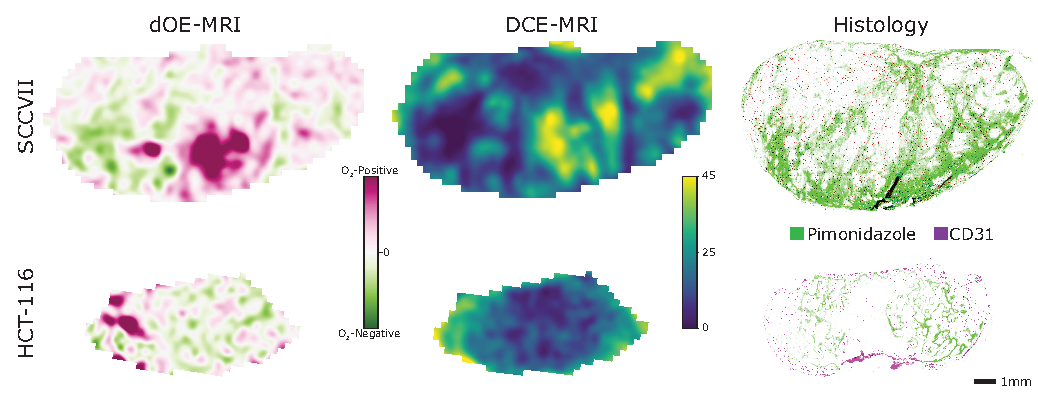
\includegraphics[width=\textwidth]{futurework/futurework-images/fig_perfusion.png} % requires the graphicx package
   \caption{\ac{dOE-MRI} maps and DCE-MRI IAUC$_{60}$maps and slice-matched histology sections of SCCVII and HCT-116 tumours. Large regions marked as purple in the \ac{dOE-MRI} maps are O$_2$-positive and also correspond to regions that have high IAUC$_{60}$ values (yellow). Green or O$_2$-negative regions from the \ac{dOE-MRI} map are often consistent with unperfused regions in the IAUC$_{60}$ (black), but there are regions of mismatch. Histology images stained with pimonidazole (green) and CD31 (purple) are shown for corresponding sections.
   \label{fig_perfusion}}
\end{figure}

\section{Adding T2* to the mix}

%%% from the grant
\todo{this is currently cribbed from the grant, it needs to be DRASTICALLY shortened, and edited for appropriateness, receptiveness, and overall style}
For a variety of reasons, the past 5-10 years have seen a gradual resurgence of oxygen-enhanced MRI and renewed interest to refine and better understand the mechanism of action.
One important strategy to elucidate the mechanism of oxygen as a contrast agent is to rely on the \acs{BOLD} effect. 
Little et al. have recently shown that simultaneous acquisition of T$_1$ and T$_2^*$ images improves the specificity of oxygen enhanced MRI~\cite{Little:2018iu}.
Here we outline how our technique using \acs{ICA} can be expanded to include T$_2^*$ imaging, and what the additional information will be used for.

T$_2^*$ imaging would utilize the Blood Oxygen Level Dependent (\acs{BOLD}) effect, which can measure shifts in hemoglobin saturation through changes in T$_2^*$ and therefore assess tumour perfusion without the need for injectable contrast agents. 
Applying an oxygen challenge also shifts the haemoglobin saturation and, thus, the T$_2^*$ signal. 
A postulated biophysical mechanisms is shown in Appendix Fig A2\todo{figure out if this is needed}. 
The expected behaviour of a joint change in T$_1$ and T$_2^*$ in response to a gas challenge, and how this can be interpreted to reflect tumour oxygenation is based on data from last year?s work by Little et al.~\cite{Little:2018iu} and Waterton et al.~\cite{OConnor:2019fc}. 

The altered T$_2^*$ provides a robust measure of areas with functioning vasculature. 
Subsequently, \acs{dOE-MRI} maps can be masked using the $\Delta$T$_2^*$ maps to exclude unperfused regions and enable improved \acs{SNR} for T$_1$-weighted signals, resulting in a completely endogenous technique to assess tumour oxygenation. 
OE-MRI T$_1$-weighted signal more directly reflects oxygen amounts in plasma and tissues and is more applicable for measuring tumour oxygenation as it relates to radiotherapy.
Without sacrificing the information obtained from T$_1$-weighted signal intensity in our current work, it is possible to extract both T$_1$-weighted signal intensity and T$_2^*$ simultaneously using a dynamic, multi-gradient echo in place of a dynamic FLASH sequence. 
We anticipate that our cycling gas challenge in combination with \acs{ICA} improvement to T$_1$-weighted oxygen enhanced imaging will also be applicable to T$_2^*$.

In preliminary work we established that a multi-gradient echo (\acs{MGE}) sequence is ideal to extend our current T$_1$ based dOE-MRI technique to also acquire dynamic T$_2^*$ weighted data.
This is because initial echoes from an \acs{MGE} sequence are T$_1$ weighted and as the echo time increases, the images become more T$_2^*$ weighted. 
The R1w-dOE-MRI map will be calculated from the signal intensity of the first gradient echo image (minimal echo time TE=2.25 ms). 
The R2*- dOE-MRI map will be created by applying ICA to the mono-exponentially fitted multi-gradient echo data at each repetition. 
Figure~\ref{MGE_schematic} outlines our approach to obtain T$_1$- and T$_2^*$-based \acs{dOE-MRI} maps from a single multi-gradient echo sequence. 
Our current experience shows that while the temporal resolution of the multi-gradient echo technique is lower, the data quality of the R1w-dOE-MRI map is not compromised until subsampling exceeds six times the original temporal resolution when compared to that obtained with a \acs{FLASH} sequence (see Figure~\ref{sec:interleave}).
Since ICA is a blind-source estimation and no input of an expected response functions is needed, one can take the successful extraction of a component that is temporally synchronized with the oxygen challenge as proof that tissue T$_2^*$ is responding to the systemic administration of oxygen. 

\begin{figure}[htbp]
   \centering
   \includegraphics[width=\textwidth]{futurework/futurework-images/grantfig4_MGE_schematic.png} % requires the graphicx package
   \caption{Schematic of the current and proposed acquisition and analysis for \acs{dOE-MRI} with combined R$_1$ and R$_2$ imaging.
   \label{MGE_schematic}}
\end{figure}

\subsection{Independent Vector Analysis}

Our application of ICA to oxygen imaging increased the sensitivity of traditional oxygen-enhanced MRI such that one can investigate oxygen response on a pixel-wise basis rather than having to average R1w signal intensity or T1 changes over regions that are defined by perfusion selection[14,25]. We are planning to investigate whether this enormous gain in statistical power can be replicated by including a further MR parameter (R2*) in a vector-based blind-source estimation adapted from an analysis technique pioneered in fMRI. The problem solved by independent vector analysis (IVA) is that observations that are vector quantities (i.e. tuples consisting of one R1-weighted signal and one R2* from the exponential fit)  are explained by a mixture  of source vectors  [26?28]:

\begin{equation}
x_i = \sum_{j}^{L} a_{ij} \circ s_j
\end{equation}

where $\circ$ indicates an element-wise product. An algorithm suggested by Rafique et al. in 2016 solves the implementation problem and makes it available as FastIVA [29]. This algorithm can be readily implemented in our current analysis framework that makes use of sklearn?s FastICA. We will use FastIVA and analyse the multi-gradient echo data acquired under Objective 1. The independent components synchronized with the oxygen-challenge paradigm will be selected for the extraction of an oxygen-challenge related component map (recall that since this is a blind-source estimation we are not providing an expected response as prior to the analysis). This map will be tested for correlation with aligned tumour sections histologically analyzed for pimonidazole.

A current approach in the use of R1-based oxygen-enhanced MRI is to use a perfusion mask from a contrast-agent injection to exclude unperfused areas. The remaining perfused regions can then be classified into oxygen-refractory and oxygen-enhancing regions[14]. The use of a contrast agent injection complicates the imaging protocol and is being resisted by clinicians[17].
We will acquire MGE data using the sequence developed under Objective 1 and create masks from baseline R2* maps as well as R2*-dOE-MRI maps. Both masks will be applied to R1-dOE-MRI maps obtained through ICA of the first-echo time course from the same MGE data. To validate this technique, we will use the injectable macromolecular contrast agent \acs{HPG-GdF} for a dynamic-contrast enhanced scan. In our previously published methodology we calculated bolus arrival time (BAT), apparent permeability?surface area product (aPS), and fractional plasma volume (fPV) [30]. BAT is a robust marker of tumour vasculature in the use of HPG-GdF. This ?perfusion? parameter map will also be used to mask areas of perfusion within which to evaluate the R1-dOE-MRI map against the histologically evaluated hypoxia marker pimonidazole. When O?Connor et al. validated the R1w-dOE-MRI method, they correlated the oxy-refractory fraction in the perfused areas (regions with positive IAUC60) with pimonidazole staining[14]. We will compare the correlations from perfusion-masked OE-MRI maps (current standard) to the correlations obtained using masking with R2* baseline and R2*-dOE-MRI maps. We will further use the parameter map calculated using IVA (vector-dOE-MRI) as a third contender in the comparison with the current standard.

%%%% End from the grant






%\begin{figure}[htbp]
%   \centering
%   \includegraphics[width=\textwidth]{futurework/futurework-images/technical_ScoredExtractions.png} % requires the graphicx package
%   \caption{Each trace plot is the extracted ICA component corresponding to the oxygen response. The components are scored by the observer from a score of 1 to 5, with 1 barely corresponding to the oxygen challenge with a lot of noise and 5 corresponding extremely well to the oxygen challenge and very little noise. Note very few animals are in the lowest group, and many more are of extraction quality 4 and 5.}
%   \label{extractions}
%\end{figure}





\endinput